%%% BEN 5' %%%

\section{Allgemeine Grundlagen}

\subsection{Die Hyperfeinstruktur}

\begin{frame}
\frametitle{Hyperfeinstruktur-Aufspaltung}
\begin{itemize}
    \item<1-> Kopplung von Kernspin $\vec{I}$ und elektronischem Gesamtdrehimpuls $\vec{J}$
    \begin{equation*}
        \vec{F} = \vec{I} + \vec{J} \qquad \qquad \abs{I - J} \leq F \leq \abs{I + J}
    \end{equation*}
    \item<2-> Energieaufspaltung
    \begin{equation*}
        \Delta E_\text{HFS} = - \vec{\mu}_I \cdot \vec{B}_J
    \end{equation*}
    \item<3-> Für benachbarte Energieniveaus
    \begin{equation*}
        \Delta E_{\Delta F = 1} (F) = A(F+1)
    \end{equation*}
    Intervallkonstante $A$
\end{itemize}
\end{frame}


\begin{frame}
\frametitle{Hyperfeinstruktur-Aufspaltung von Rubidium}
\setbeamerfont{myfont}{size*=80}
\usebeamerfont{myfont}

\begin{figure}
    \centering
    \def\svgwidth{\textwidth}
    \input{../img/termschemahyperfein.pdf_tex}
    \caption{Hyperfeinstrukturaufspaltung der D$_1$-Linie von \rb{85} und \rb{87}.}
\end{figure}
\end{frame}


\begin{frame}
\frametitle{Hyperfeinstruktur-Aufspaltung - Übergänge}
\setbeamerfont{myfont}{size*=80}
\usebeamerfont{myfont}

\begin{figure}
    \centering
    \def\svgwidth{\textwidth}
    \input{../img/termschemahyperfein_linien.pdf_tex}
    \caption{Hyperfeinstrukturaufspaltung der D$_1$-Linie von 
    \rb{85} und \rb{87}.}
\end{figure}
\end{frame}

 


\begin{frame}
\frametitle{Hyperfeinstruktur-Aufspaltung - Spektrallinien}
\setbeamerfont{myfont}{size*=80}
\usebeamerfont{myfont}

\begin{figure}
    \centering
    \def\svgwidth{\textwidth}
    \input{../img/HFSspect_theo.pdf_tex}
    \caption{Spektrallinien der Hyperfeinstruktur des ${}^2\text{S}_{1/2}$\,-\,${}^2\text{P}_{1/2}$\,-\,Übergangs
    von \rb{85} und \rb{87}.}
\end{figure}

\end{frame}

\begin{frame}
\frametitle{Zeeman-Aufspaltung der Hyperfeinstruktur}
\begin{itemize}
    \item<1-> ohne Magnetfeld: Niveau ist $(2F+1)$-fach entartet
    \begin{equation*}
        F_z = m_F \hbar \qquad \qquad -F \leq m_F \leq F
    \end{equation*}
    \item<2-> mit äußerem Magnetfeld $\vec{B}_0$: Zeeman-Aufspaltung
    \item<3-> Für benachbarte Energieniveaus
    \begin{equation*}
        \Delta E_\text{HFS}^\text{Zeeman}(\Delta m_F = 1) = \frac{g_J \mu_B}{2 \left( I + \frac{1}{2} \right) } B_0
    \end{equation*}
    Bohrsches Magneton $\mu_B$, Landé-Faktor $g_J$
\end{itemize}
\end{frame}

\begin{frame}
\frametitle{Zeeman-Aufspaltung der Hyperfeinstruktur}

\setbeamerfont{myfont}{size*=80}
\usebeamerfont{myfont}

\begin{figure}
    \centering
    \def\svgwidth{\textwidth}
    \input{../img/termschema.pdf_tex}
    \caption{Zeeman-Aufspaltung der Hyperfeinstruktur von \rb{85} und \rb{87}.}
\end{figure}

\end{frame}




%%% MORITZ 2.5' %%%

\subsection{Die Laserdiode}

\begin{frame}
\frametitle{Laserdiode - Aufbau zur Charakterisierung}
\setbeamerfont{myfont}{size*=80}
\usebeamerfont{myfont}
\begin{figure}
    \centering
    \def\svgwidth{\textwidth}
    \input{../img/aufbauLaser.pdf_tex}
    \caption{Aufbau zur Messung der $P$-$I$-Kennlinie der Laserdiode.}
\end{figure}
\usebeamerfont{standard}
\begin{itemize}
  \item \textbf{Peltierelement:} Temperaturstabilisierung der Laserdiode
  \item \textbf{Laserdiode:} Erzeugung von linear polarisiertem kohärenten Licht mit $\lambda=500$\,nm
  \item \textbf{Neutraldichtefilter:} Abschwächung der Laserintensität
  \item \textbf{Photodiode:} Messung der Laserintensität
\end{itemize}
\end{frame}

\begin{frame}
\frametitle{Laserdiode - $P$-$I$-Kennlinie}

\begin{figure}[H]
    \begin{center}
        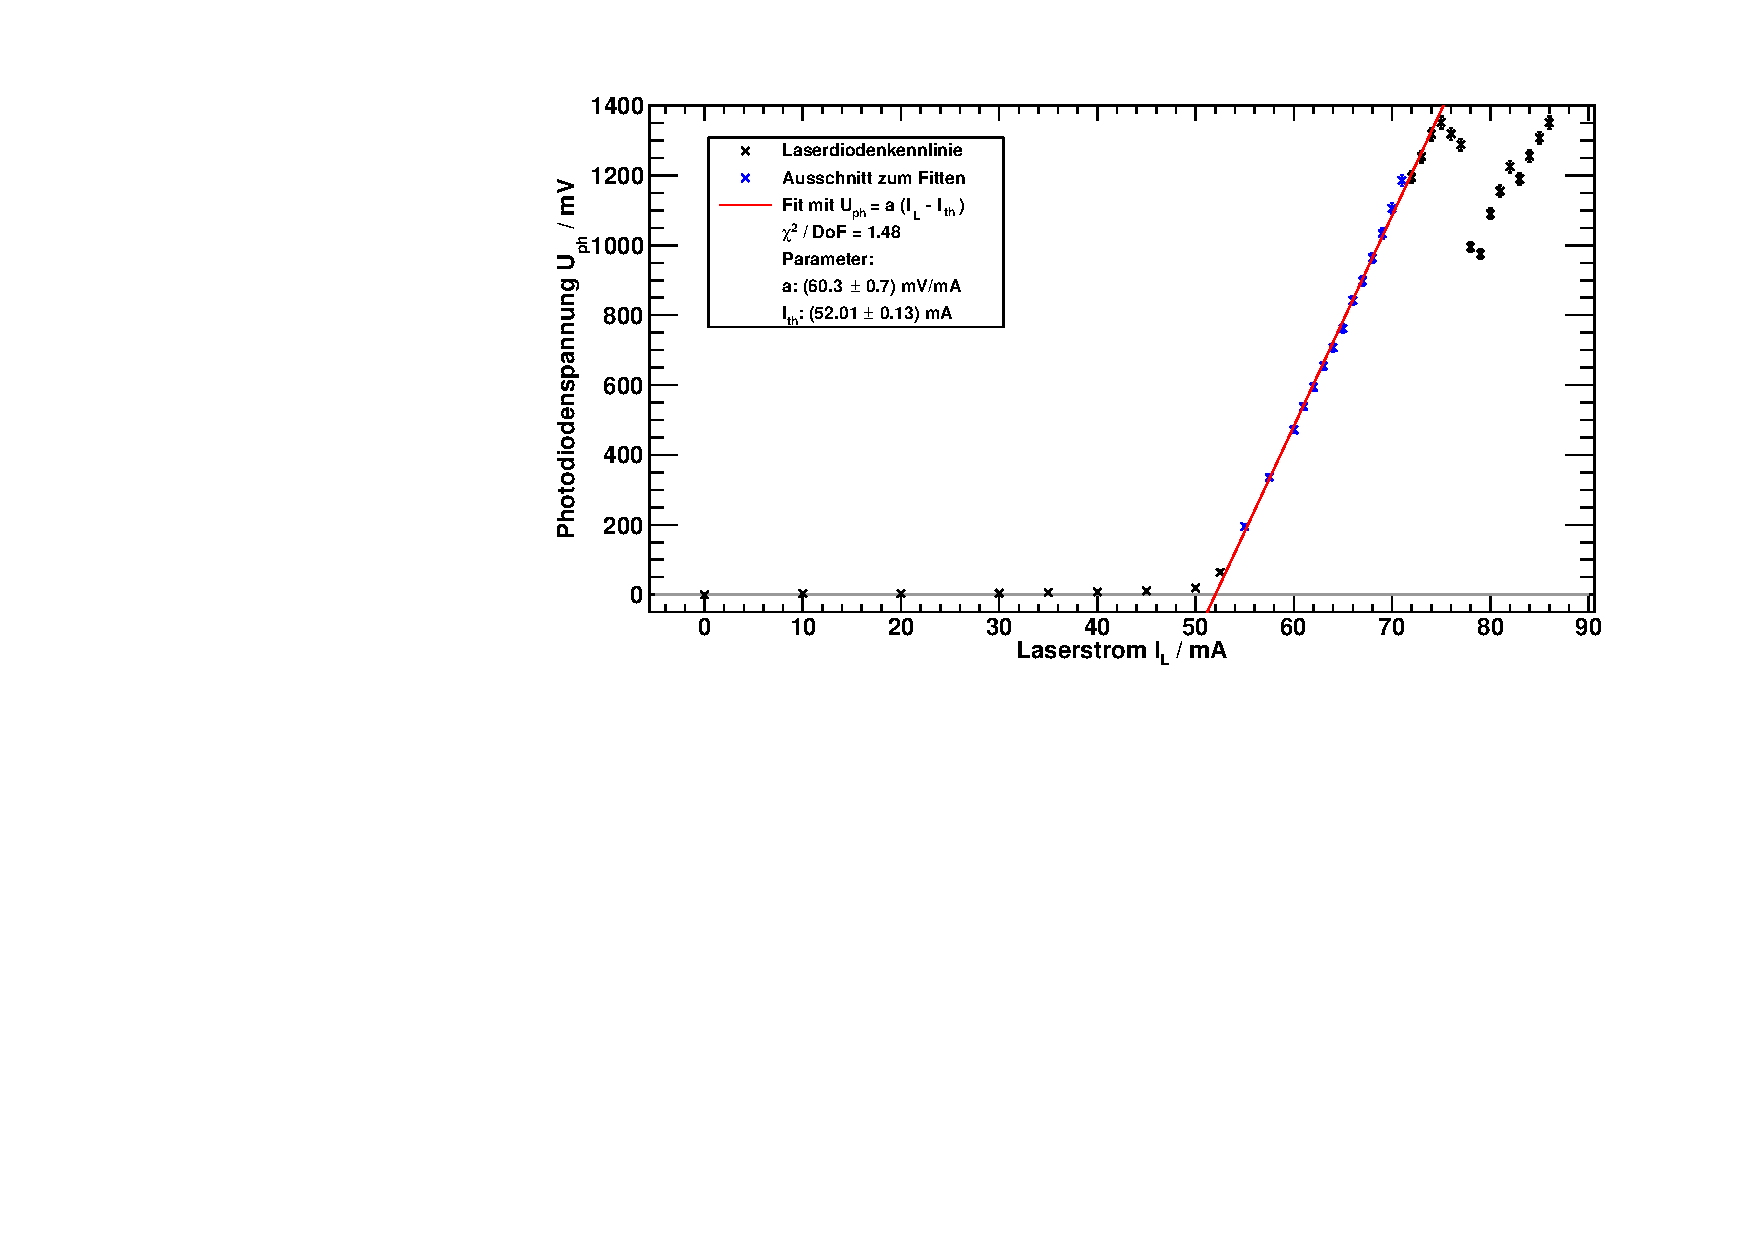
\includegraphics[width=\textwidth]{../img/diodenkennlinie.pdf}
        \caption{$P$-$I$-Kennlinie der im Versuch verwendeten Laserdiode.}
    \end{center}
\end{figure}
\end{frame}

\begin{frame}
\frametitle{Laserdiode - Aufbau zur Charakterisierung}
\setbeamerfont{myfont}{size*=80}
\usebeamerfont{myfont}
\begin{figure}
    \centering
    \def\svgwidth{\textwidth}
    \input{../img/aufbauEtalon.pdf_tex}
    \caption{Aufbau zur Identifikation von Modensprüngen der Laserdiode.}
\end{figure}
\usebeamerfont{standard}
\begin{itemize}
  \item \textbf{Etalon:} Transmissionsmaxima mit bekanntem Abstand
\end{itemize}
\end{frame}


\begin{frame}
\frametitle{Laserdiode - Frequenzmodulation}
\begin{figure}[H]
    \begin{center}
        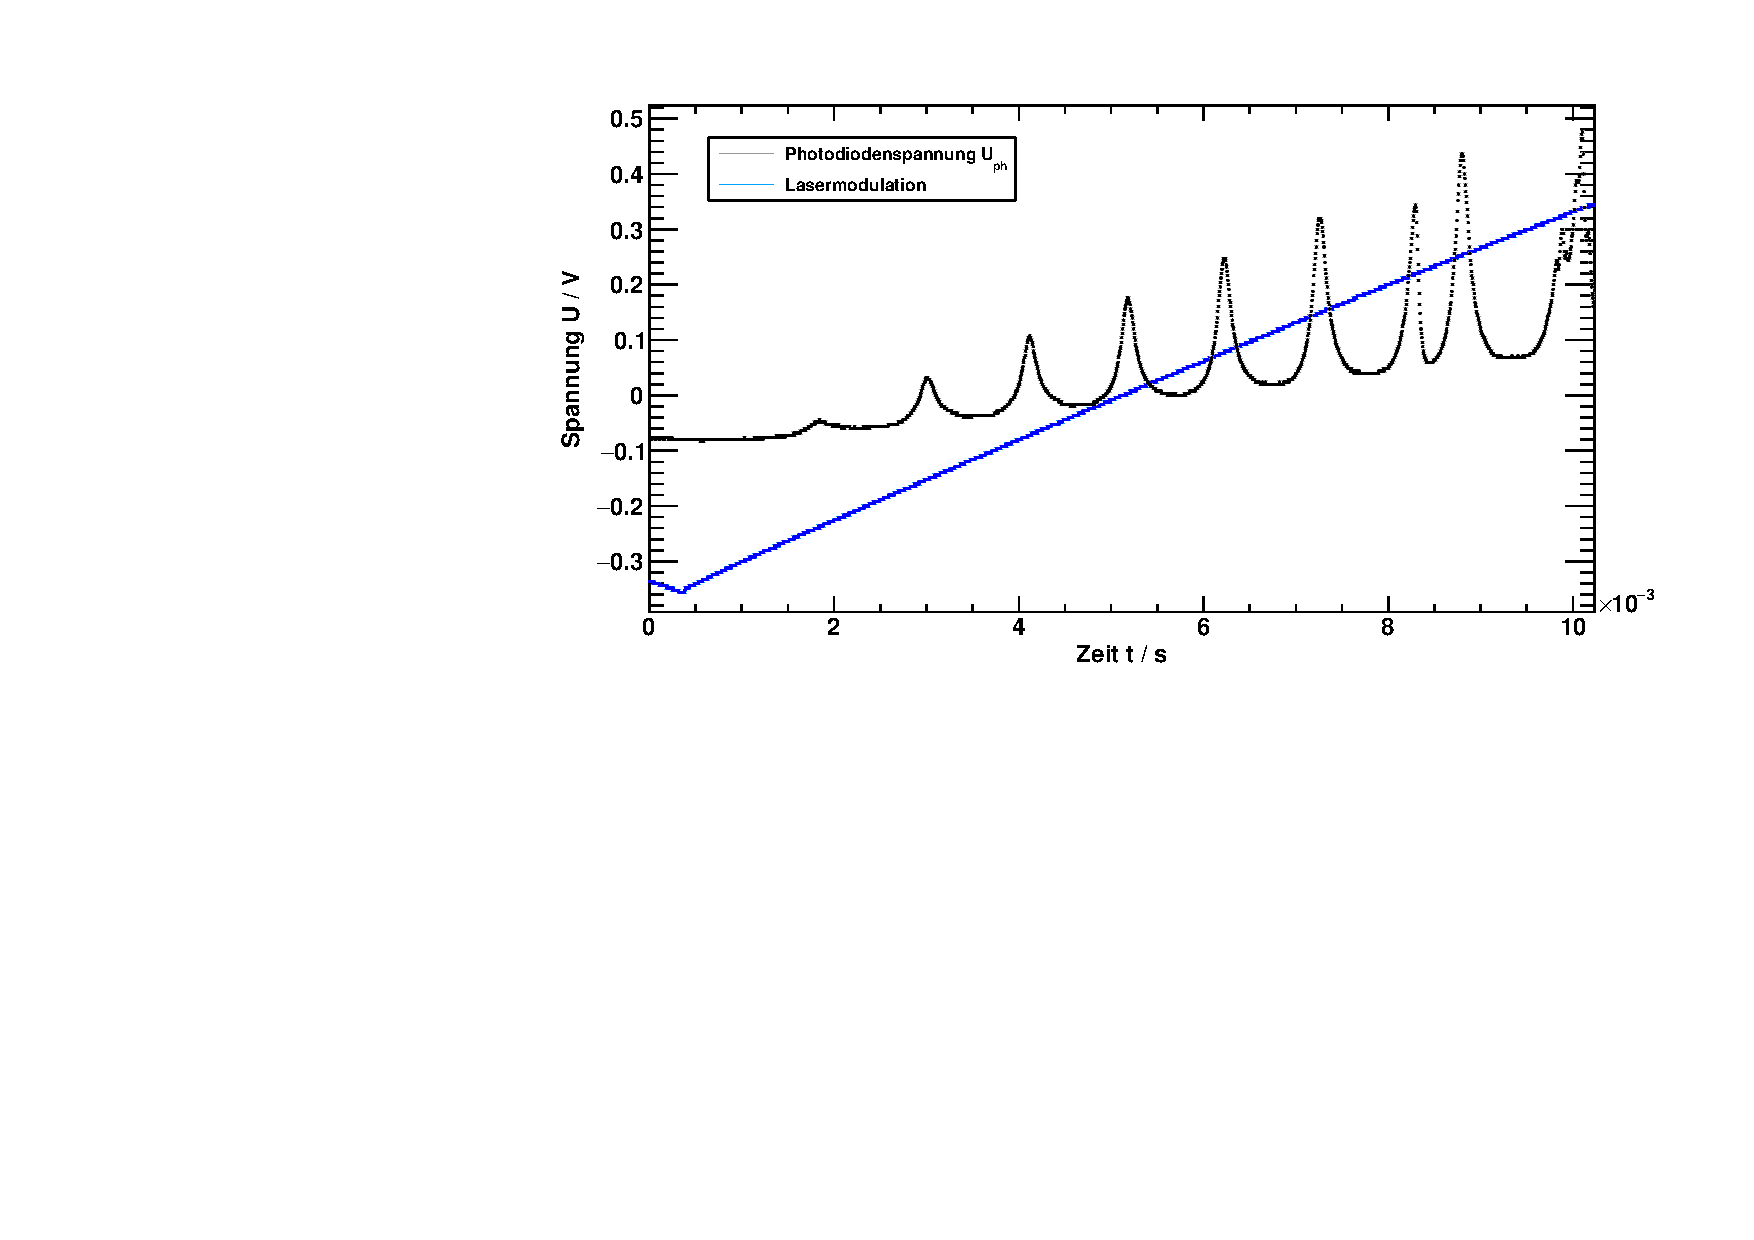
\includegraphics[width=\textwidth]{../img/up-etalon_zoom.pdf}
        \caption{Frequenzabhängige Transmission des Laserlichts durch das Etalon.}
    \end{center}
\end{figure}
\end{frame}


\begin{frame}
\frametitle{Laserdiode - Frequenzmodulation}

\begin{figure}[H]
    \begin{center}
        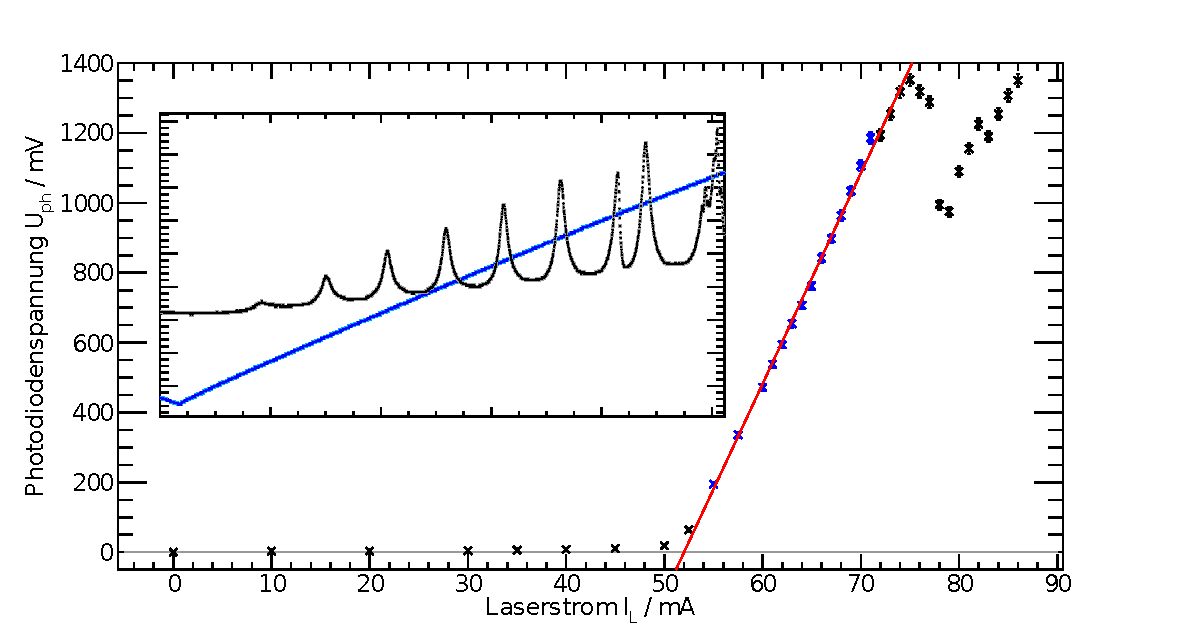
\includegraphics[width=\textwidth]{../img/diodenkennlinie+etalonspect.pdf}
        \caption{Vergleich von Frequenz und Leistung der Laserdiode.}
    \end{center}
\end{figure}
\end{frame}



